% How we create the data
% Explain the set-up of the algorithm
% Explain the code, refer to Intro / remember equations 
% lave figur der beskriver hele vores Architecture / model set up

\section{Materials and Methods}

\subsection{Data Creation and Reprocess}

\textbf{Sequences}:  The model can be trained on a single or multiple sequences. However, the length must be constant for multiple sequences. The implementation took starting point in the unfair casino where an input sequence is a representation of a number of die tosses. However, multiple types of sequences could be used.

\noindent
\textbf{Sequence encoding:} The sequence used in the HMM must be encoded so that each symbol in the sequence $\in [0,n-1]$ where n denotes the number of unique symbols in the sequence. This allows the model to use the symbol encoding as index for the emission matrix described in \autoref{subsec:BW}. Thus, in the case of a die toss the results will be encoded as a number between 0 and 5.

\noindent
\textbf{Generation of sequences}: In order to test our implementation a small sequence generator was created which generates a sequence of specified length using set parameters for initial distribution, transition, and emission matrices.


\subsection{Baum-Welch} \label{subsec:BW}
\subsubsection{Initial model parameters}
The Baum-Welch algorithm has to be initialised with values for the emission, transition and initial state matrices. The starting values are important as the BW algorithm will not be able to escape local extrema. In our case we chose to initialise the model with equal rates for all transition events and equal probability for intial state. Furthermore, the emission matrix was initialised with uniformly distributed random values for the emission rates normalised so they summed to one within each state. 

\subsubsection{Forward algorithm}\label{method.forward}
The forward algorithm describes the probability of aligning a sequence to the model from the start up to a given position i in state k.  This is given by the sum of probability of reaching the position and the state from all paths. The probabilities are then calculated recursively and stored in the $\alpha$ matrix. The formula is given in \autoref{eq:fw_sum} as the sum version and in \autoref{eq:fw_linalg} as the linear algebra implementation used in the project. The linear algebra implementation using numpy arrays is faster and appears more elegant.

\begin{equation}
    \alpha_{k}(i) = b_k(x_i) \cdot \sum_{l} \alpha_l(x_{i-1}) \cdot a_{lk}\\
    \label{eq:fw_sum}
\end{equation}

\begin{equation}
    \alpha[i,k] = (\alpha[i-1]\textbf{.}A[:,k]) \cdot B[k, x_i]\\
    \label{eq:fw_linalg}
\end{equation}
where A = transition matrix, B = emission matrix, and x the observed sequence.\\

\noindent
Note, that the summed values for all k for i=N is the probability of aligning an observed sequence to the HMM.

\subsubsection{Backward algorithm}\label{method.backward}
The backward algorithm determines the probability of aligning a sequence X from i+1 to N to the HMM from a starting state k. The values all positions i and states k are calculated backwards from i=N where the probability is given as 1 and the recursively calculated values are stored in matrix $\beta$. Like the forward algorithm, the standard formula is given in \autoref{eq:bw_sum} and the linear algebra implementation used in the project is given in \autoref{eq:bw_linalg}.

\begin{equation}
    \beta_{k}(i) = \sum_l t_{kl} \cdot b_l(x_{i+1}) \cdot \beta_l(i+1)
    \label{eq:bw_sum}
\end{equation}

\begin{equation}
    \beta[i,k] = (\beta[i+1] \cdot B[:,x_{i+1}])\textbf{.}B[k,:]
    \label{eq:bw_linalg}
\end{equation}

\subsubsection{Updating parameters} \label{seq:upt_par}

From the $\alpha$ and $\beta$ matrices we can now determine how to update the transition and emmision matrix as well as the initial distribution of states. Initially two temporary variables are calculated; $\gamma$ which describes the probability of being in state \textit{i} and time \textit{t} and $\xi$ describing the probability of being in state \textit{i} at time \textit{t} and \textit{j} at times \textit{t+1}. The equations for $\gamma$ $\xi$ is given in \autoref{eq:upt_ga} and \autoref{eq:upt_xi}.

\begin{equation}
    \gamma_i(t) = \frac{\alpha_i(t) \cdot \beta_i(t)}{\sum_{j=1}^M \alpha_j(t)\cdot\beta_j(t)}
    \label{eq:upt_ga}
\end{equation}

\begin{equation}
    \xi_i(t) = \frac{\alpha_i(t)\cdot a_{ij} \cdot \beta_j(t+1) \cdot b_j(x_{i+1})}{\sum_{k=1}^{M} \sum_{w=1}^M \alpha_k(t) \cdot a_{kw} \cdot \beta_w(t+1) \cdot b_w(y_{t+1})}
    \label{eq:upt_xi}
\end{equation}

For the our implementation the above equation was redone using linear algebra.
Note that xi has the dimentions (M,M, T-1) where M is the number of hidden states and T the length of each sequence.
\begin{equation}
    \xi[t,:, i] = \frac{\alpha[i,t] \cdot A[t,:] \cdot B[:, x_{i+1}].T \cdot \beta[i+1,:].T}{(\alpha[i,:]\textbf{.}(A \cdot B[:, x_{i+1}].T)\textbf{.}\beta[i+1, :]}
\end{equation}

\noindent
$\gamma$ is then given by taking the sum of $\xi$ with respect to the second axis.\\

\noindent
With the temporary parameters the transition, emission, and intial distribution matrices can be updated as seen below. 
Note, that the standard formula is defined first followed by our implementation.\\

\textbf{Initial distribution:}
\begin{equation}
    \pi_i = \gamma_i(1)
\end{equation}

\textbf{Transition matrix}
\begin{equation}
    a_{ij} = \frac{\sum_{t=1}^{T-1} \xi_{ij}(t)} {\sum_{t=1}^{T-1} \gamma_i(t)}
\end{equation}

\textbf{Emission matrix}
\begin{equation}
    b_i(v_k) = \frac{\sum_{t=1}^T 1_{y_t=v_k} \gamma_i(t)}{\sum_{t=1}^T \gamma_i(t)} \\
\end{equation}

where $1_{y_t=v_k} = 1$ if ${y_t=v_k}$ and otherwise 0\\

\noindent
\textbf{Implementation used in this paper:}\\

\textbf{Initial distribution:}
\begin{equation}
    \pi^* = \gamma[:,0]
\end{equation}

\textbf{Transition matrix}
\begin{equation}
    A^* = \frac{\sum_t^{T-1} \xi[:,:,t]}{\sum_t^{T-1} \gamma[:,t]} 
\end{equation}

\textbf{Emission matrix}
\begin{equation}
    B^*[:,v_k] =  \frac{\sum_{t=1}^{T} \gamma[:,y_t=v_k]}{\sum_t^{T} \gamma[:,t]}
\end{equation}

\subsubsection{Multiple sequences}
The formula given in Section \ref{seq:upt_par} are valid if the input consists of a single sequence. However, if the input consists of multiple sequences the update one applies to the parameters must take into account the values for $\gamma$ and $\xi$ for the individual sequences. 

Thus to handle multiple sequences a the $\alpha$ and $\beta$ matrices are calulated for each sequence and from them the individual $\gamma$ and $\xi$ values. Then the update formulas are changed so that the nominator is summed for each sequences and the denominator is summed for each sequence before the fraction is solved. The equations for multiple sequences with the linear algebra implementation are given below: \\

\textbf{Initial distribution:}
\begin{equation}
    \pi^* = \frac{\sum_{r=1}^R\gamma_r[:,0]}{R}
\end{equation}

\textbf{Transition matrix}
\begin{equation}
    A^* = \frac{\sum_{r=1}^R\sum_t^{T-1} \xi_r[:,:,t]}{\sum_{r=1}^R\sum_t^{T-1} \gamma_r[:,t]} 
\end{equation}

\textbf{Emission matrix}
\begin{equation}
    B^*[:,v_k] =  \frac{\sum_{r=1}^R \sum_{t=1}^{T} \gamma_r[:,y_t=v_k]}{ \sum_{r=1}^R \sum_t^{T} \gamma_r[:,t]}
\end{equation}

\textbf{Note}: The sum over R sequences are performed in an element wise manner on the matrices.

\subsection{Rescaling}

With longer sequences $\alpha$ and $\beta$ values can become very small underflow is therefor a risk. To avoid underflow a normalisation factor Z is calculated at each time step and used to normalise both $\alpha$ and $\beta$ matrices. The equations for the normalisation are given below:

\begin{align}
    Z(t) = \sum_{i=1}^M \alpha_i(t) \\
    \alpha^*_i(t) = \frac{\alpha_i(t)}{Z(t)} \\
    \beta^*_i(t) = \frac{\beta_i(t)}{Z(t)}
\end{align}


\subsection{Model Performance Evaluation}

The model can be evaluated in two distinct ways considering whether you are testing the models performance to pick up a known underlying pattern or that you are trying to learn an unknown pattern. If the pattern is known it an approach to compare the estimated parameters and the true parameters would be to calculate the mean squared error (MSE) between the parameters. If the true parameters are not know, as is the case for most real-world application using the negative log likelihood of the observed sequence given the model will most likely be the best approach. 

The negative log-likelihood is in our implementation calculated on a separate test set. First the model is trained on a training set of sequences, then the forward algorithm is run for each sequence in the test set, the probability of the sequence for all states are log transformed and summed. This gives log likelihood for each sequence which is then averaged. The formula is given below:

\begin{equation}
    log(likelihood)_{avg} = \frac{\sum_{r=1}^R \sum_k\log(\alpha_r[k,-1]) }{R}
\end{equation}

From the log likelihood one can then choose which trained model to use, as some of the trained models will most likely get stuck on poor local extrema. \\

\noindent
With regards to testing the model against a known set of parameters it is important to note that order of the states are arbitrary in the output of the Baum-Welch model. Therefore, to compare with known parameters one would need to try all permutations of the output with regards to state order against the true parameters and then the true MSE would be the smallest.

\subsection{Model Ensemble}

To increase the robustness of trained models this implementation allows for bagging a number of trained models into an ensemble. Thus, the ensemble parameters will be an average of the parameters for each run. However, as noted in previous section the order of states is arbitrary. Therefore, it is necessary to rotate all of the parameter matrices from the individual runs to have the same ordering of states.

This is done by setting one model as reference and then permutating the order of states for all other models and selecting the permutation for each model with the smallest MSE to the reference model. The reference model is chosen as the model with the small negative log likelihood. 


% MSE
% After model run, calculate forward on sequences with found model parameters to test how probable our our data is, given the found parameters


\subsection{Overview of Model Architecture} 
An overview of our model architecture is visualised in \autoref{fig:set_up}. First, transition, emission, and state distribution matrices are simulated to resemble the unfair casino problem. These matrices are then used to create a number of artificial sequences representing die tosses. The majority of the sequences are used as training data, whereas a smaller part of the sequences are used as testing data. 

In order to test the robustness of the model, seven models are run independently on the same training data, having different initiations of the parameters. This gives seven different sets of optimal model parameters. \autoref{fig:baum_w} visualises our setup of the Baum-Welch algorithm that yields the optimal model parameters. An ensemble model was also computed based on the seven models.

Two different approaches were used to evaluate the model performance. (1) The mean-squared-error (MSE) between the estimated parameters and the simulated parameters is calculated for each model and for the ensemble model. (2) The average negative log-likelihood of the sequences in the test data is computed by running the sequences through the forward algorithm, for each of the models and for the ensemble model. The evaluation measurements are finally plotted.

\begin{figure}[H]
    \centering
    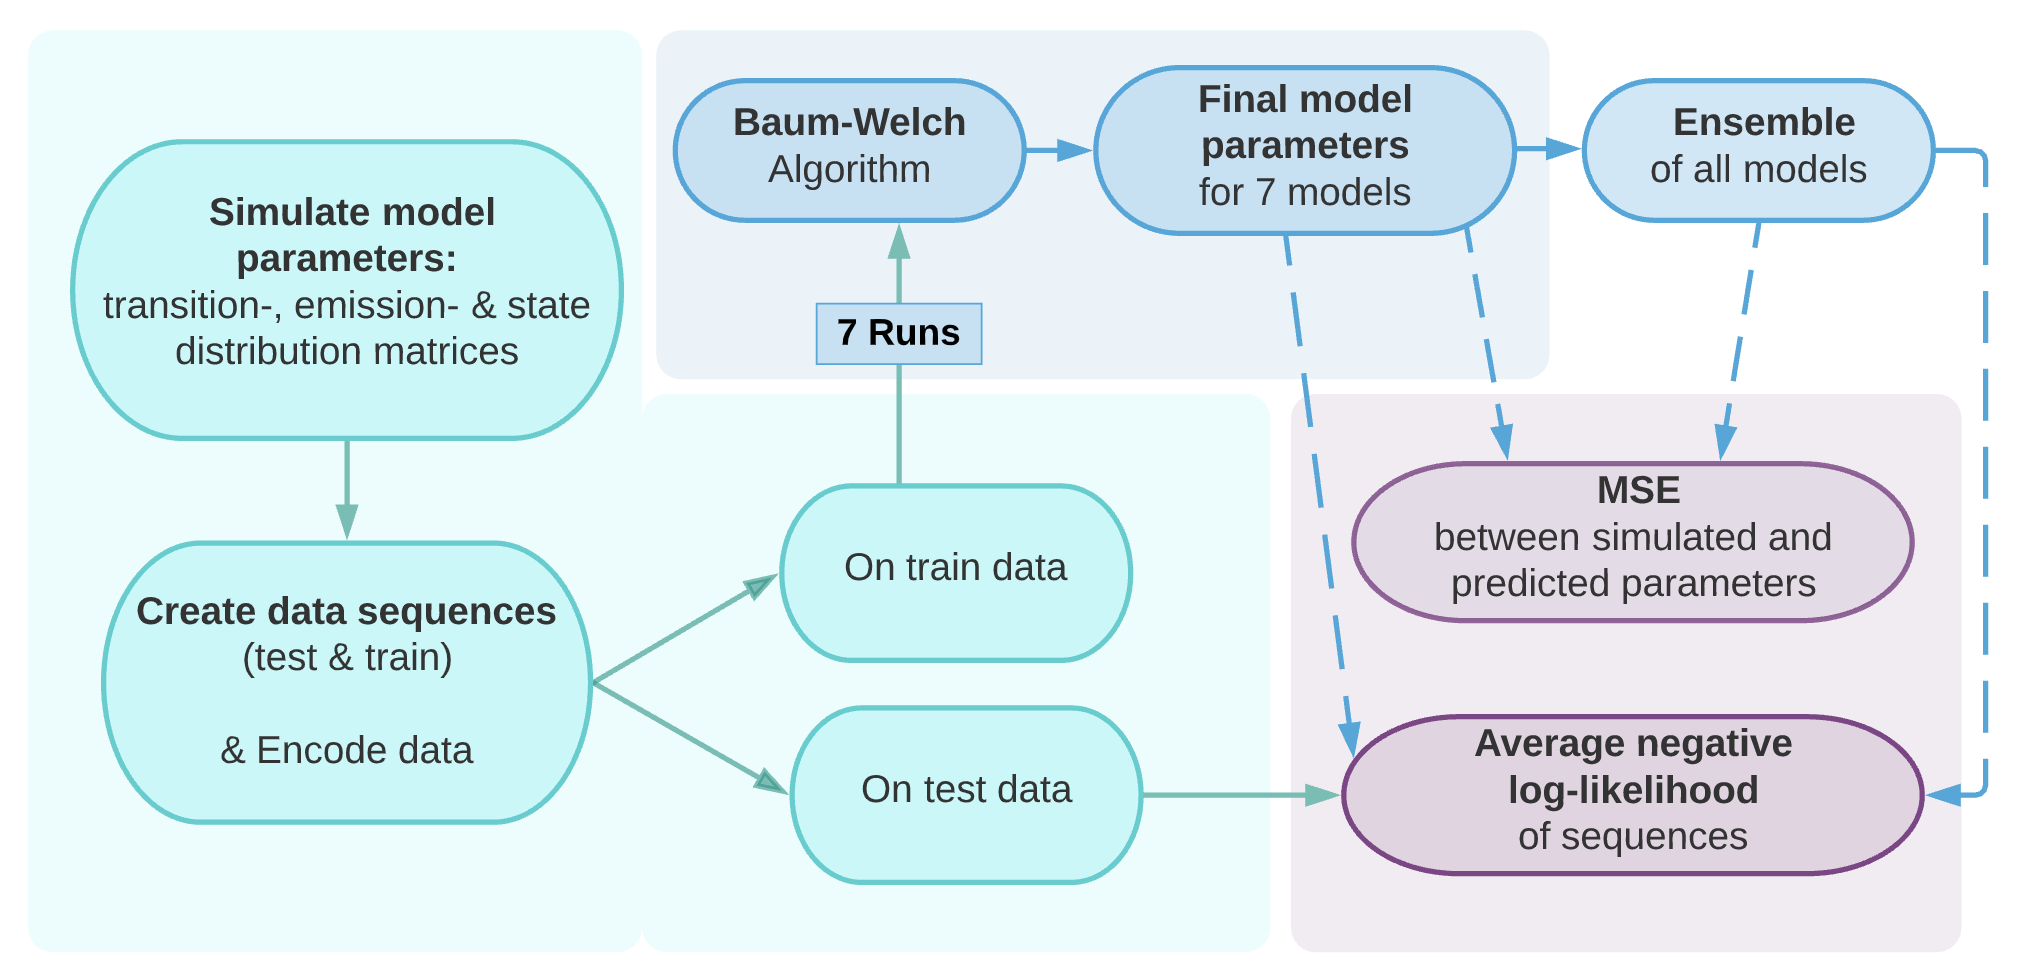
\includegraphics[width = 0.95\textwidth]{fig/Overall_setup.png}
    \caption{Overview of the model set up. \textit{Homemade}.}
    \label{fig:set_up}
\end{figure}

An overview of the Baum-Welch algorithm set-up is visualised in \autoref{fig:baum_w}. 
\begin{figure}[H]
    \centering
    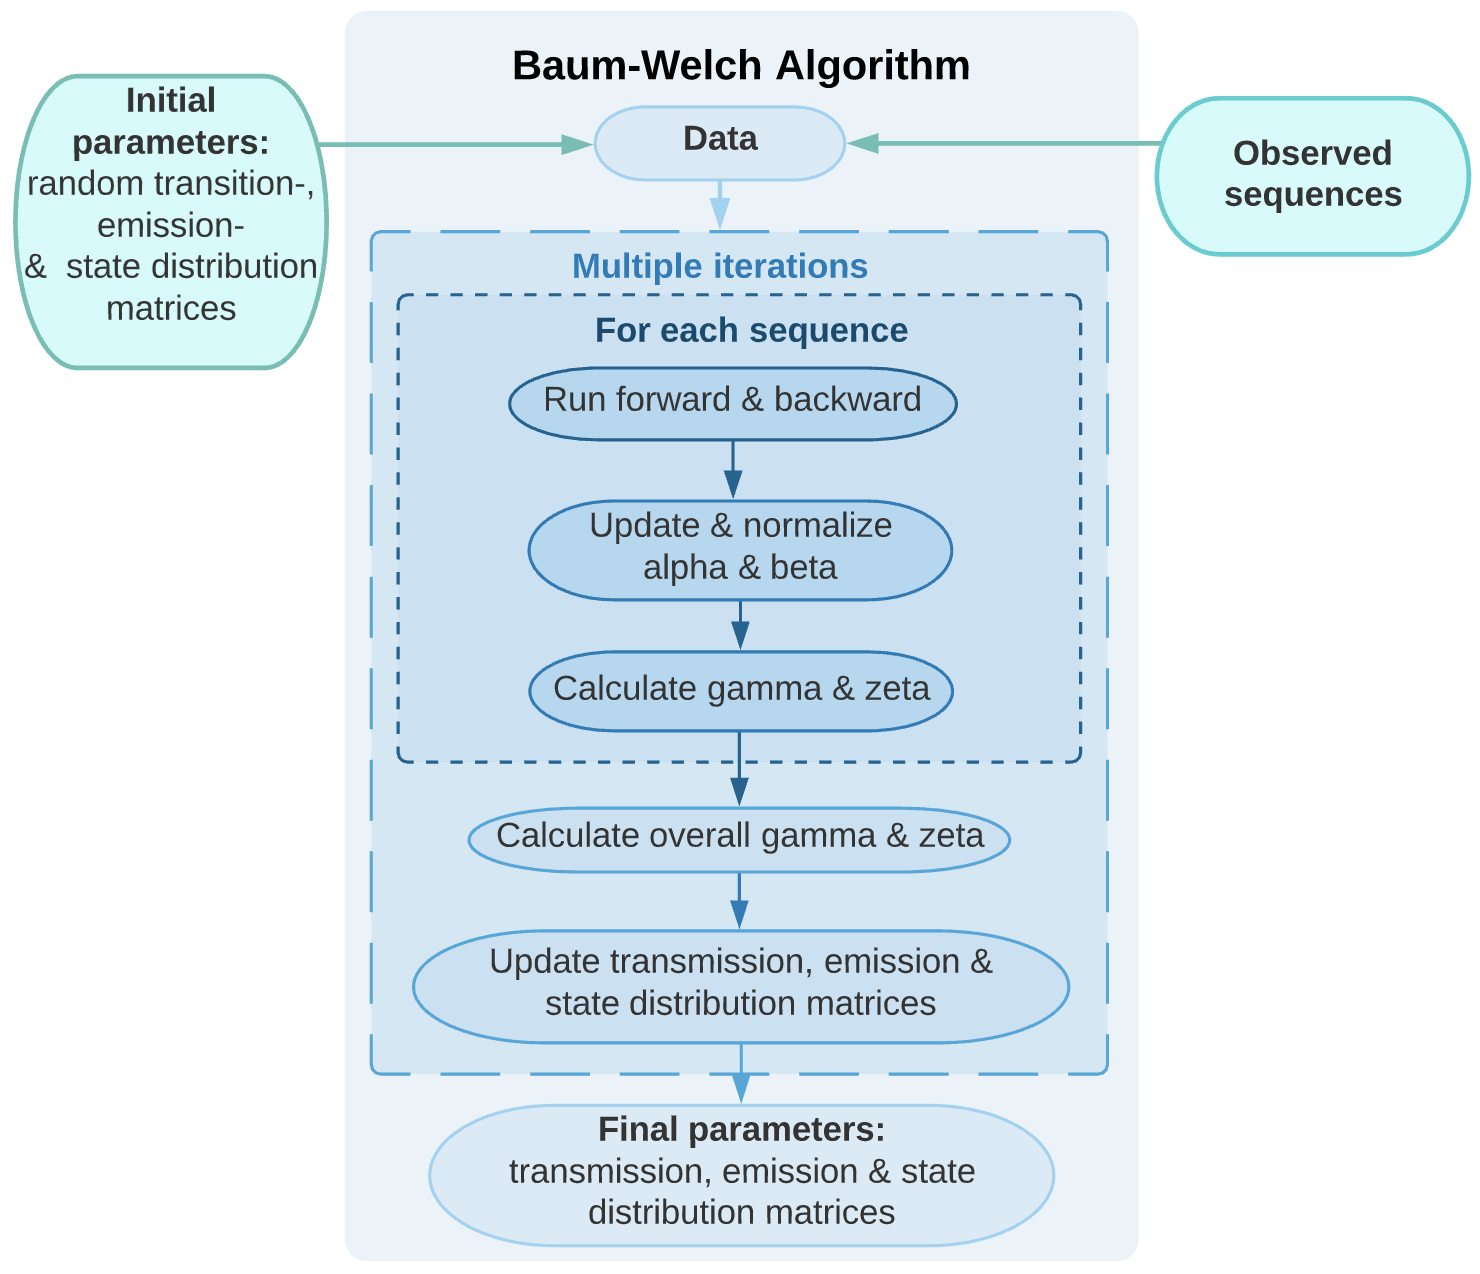
\includegraphics[width = 0.9\textwidth]{fig/baum_welch.png}
    \caption{Overview of the Baum-Welch algorithm. \textit{Homemade}.}
    \label{fig:baum_w}
\end{figure}

% ved ikke om vi behøver flere kommentarer til BW?
